\documentclass[ a4paper,
                oneside,
                toc=bibliography,
                toc=listof
                ]{scrbook}


% set the language here. Last language is the main language. Use `ngerman` (= new german) for German texts.
\usepackage[ngerman, english]{babel}
% \usepackage[english,ngerman]{babel} % If your text mainly is in German.



% general math support
% consider using bracket environments for inline math, i.e. \(x_2^2 + \sqrt{\gamma}\) instead of $$.
% for numbered equations in their own line, use e.g. the array environment. 
\usepackage{amsmath, amssymb}

% bold math package. Set matrices and vectors with \bm{v}
\usepackage{bm}

% beautiful table environments (see https://ctan.org/pkg/booktabs)
\usepackage{booktabs}

% multi page table. Your list of symbols may need this
\usepackage{longtable}

% consistent acronym definitions and usage. You may want to use the glossaries package instead, which is more powerful, but more complex to handle.
\usepackage[printonlyused, smaller]{acronym}

% for multiple plots in one figue, e.g. Fig 1.a and Fig 1.b
% https://en.wikibooks.org/wiki/LaTeX/Floats,_Figures_and_Captions#Subfloats
\usepackage{subcaption}

% provides \FloatBarrier to prevent floats past some point.
\usepackage{placeins}

% For vector graphics and MATLAB figures, you may try TikZ:
% There is also tikz-uml for UML diagrams
\usepackage{tikz}
\usepackage{pgfplots}

\pgfplotsset{
    compat = newest,
	grid=major,
	every axis plot/.append style={very thick},
}

% block diagrams with tikz
\usetikzlibrary{calc,fit, positioning,arrows.meta}
\tikzset{>={Latex[width=2mm,length=2mm]}} % more visible default arrow heads
\tikzstyle{block} = [draw=black, fill=white, rectangle, align=center, minimum height=2em, minimum width=3em]
\tikzstyle{sum} = [draw, circle, node distance=1cm]

% global matlab2tikz options for exporting MATLAB plots
% https://github.com/matlab2tikz/matlab2tikz
\newlength\figureheight 
\newlength\figurewidth 
\setlength\figureheight{3cm} 
\setlength\figurewidth{0.7\textwidth}


% If you want to use colors, we already defined some for you (university corporate design)
\RequirePackage{xcolor}

\definecolor{UStuttDarkBlue}{RGB}{0,81,158}
\definecolor{UStuttLightBlue}{RGB}{0,190,255}
\definecolor{UStuttDarkGreen}{RGB}{59,140,122}
\definecolor{UStuttLightGreen}{RGB}{125,155,101}
\definecolor{UStuttDarkOrange}{RGB}{228,175,52}
\definecolor{UStuttLightOrange}{RGB}{236,218,145}


% for code listings, you can e.g. use the "listings" package (http://texdoc.net/texmf-dist/doc/latex/listings/listings.pdf):
\usepackage{listings} 
\usepackage{scrhack} % if you load listings together with scrbook etc., then load this fixing package as well

\lstset{
  captionpos=b,
  commentstyle=\color{UStuttDarkGreen},
  frame=single,	                   % adds a frame around the code
  keepspaces=true,
  %keywordstyle=\color{UStuttDarkBlue},
  showspaces=false,
  showstringspaces=false,          % underline spaces within strings only
  showtabs=false,
  stringstyle=\color{UStuttDarkBlue},
  tabsize=2
}


% This class does the ISW styling for you (together with scrbook).
%
% It handles the following:
% - Proper input and font encoding (Just type, don't care about the LaTeX compiler you use or how to type German umlauts)
% - Fonts with ligatures and kerning (Tex Gyre fonts are used, part of every LaTeX installation, text is nice to read)
% - Bibliography styling for biblatex (declare your bibliography file and you are ready to go)
% - Provide command for title page (\makeISWtitle) and declaration of originality ( \declarationOfOriginality)
% - Loads packages "biblatex" and "graphics"
\usepackage[
    type=MA, % BA, MA, FA, SA (old), bachelorproject
]{iswthesis}

% hyperref provides hyperlinks within the document, but also auto-naming.
% E.g. when referencing, instead of typing "Figure~\ref{fig:XY}" try "\autoref{fig:XY}".
% You may want to use `clevceref` instead of using \autoref in the hyperref package, which has slightly more possibilities.
\PassOptionsToPackage{pdfpagelabels}{hyperref}
\usepackage{hyperref}  % backref linktocpage pagebackref
\pdfcompresslevel=9
\pdfadjustspacing=1

\hypersetup{%
    %draft, % = no hyperlinking at all
    %colorlinks=true,
    colorlinks=false, 
    linktocpage=false, pdfborder={0 0 0},%
    breaklinks=true, pdfpagemode=UseNone, pageanchor=true, pdfpagemode=UseOutlines,%
    plainpages=false, bookmarksnumbered, bookmarksopen=true, bookmarksopenlevel=1,%
    hypertexnames=true, pdfhighlight=/O,%nesting=true,%frenchlinks,%
    %urlcolor=Black, linkcolor=Black, citecolor=Black, %pagecolor=Black,%
} 


% Your own commands (https://en.wikibooks.org/wiki/LaTeX/Macros):
% Consider defining your own commands for often used terms, e.g.

% Real numbers symbol
\newcommand{\R}{\mathbb{R}}

% Transpose of vector or matrix (upright)
\newcommand{\T}{\mathrm{T}}

\newcommand{\mustbe}{\ensuremath{\stackrel{!}{=}}}

% short matrix environment. Instead of typing \begin{bmatrix} 1 & 2 \\ 3 & 4 \end{bmatrix} you can now use as well \bmat{1 & 2 \\ 3 & 4}
\newcommand{\bmat}[1]{ \ensuremath{\begin{bmatrix} #1 \end{bmatrix}} }

% partial derivative: \partfrac{^2}{x^2} yields ∂²/∂x²
\newcommand{\partfrac}[2]{ \ensuremath{\frac{\partial #1}{\partial #2}} }

% upright "d" for differentiation
\newcommand{\ddiff}{\ensuremath{\mathrm{d}}}

% d/dt
\newcommand{\ddt}{\ensuremath{\frac{\ddiff}{\ddiff t}}}


\usepackage{algpseudocode}

% font size for captions 
\usepackage[font=footnotesize]{caption}        % small, footnotesize, scriptsize, or large


% Path to .bib file for BibLatex
\addbibresource{bibliography.bib}
% \addbibresource{someOtherBibFile}

\author{Frederik Omlor}
\placeOfBirth{Backnang}
\address{Karl-Krische-Straße 40, 71522 Backnang, Germany}
\major{Computer Science and Media}
\title{Mesh Shading Optimization in Voxel-Based Volumetric Rendering}
\titleTranslated{Mesh Shading Optimierung in Voxel-Based Volumetric Rendering}
\matrnr{45044}
\date{\today}
\supervisor{Wilhem Lorin Atzberger}
\professor{Prof. Dr. Stefan R. Radicke \& Dr. Andreas Stiegler}

\begin{document} 
    \frontmatter
    \makeISWtitle

	\cleardoublepage
	\setcounter{page}{1} % start at page (i) after title page
    \declarationOfOriginality

    \chapter{Acknowledgements}

This work would not have been possible without the help of many great people, who I want to thank for their 
participation and support. First of all, my gratitude goes to my supervisors Professor Dr. Stefan Radicke 
and Dr. Andreas Stiegler for supporting my work from the day I approached them. Thank you for providing 
valuable input and discussing topic ideas while always giving me the freedom to pursue my interests. In 
this context I also want to thank everyone who helped me achieve my goals during my studies and all the 
people at Hochschule der Medien for making this possible. \\

\noindent
I want to specifically thank my external supervisor Wilhelm Lorin Atzberger, who I met at Nordic Game Jam 
in April 2024. I never expected finding success in my search for external support just a few weeks before 
starting to work on the thesis. I want to thank you for being spontaneous, for listening and for your 
extraordinary support. Thank you for spending so many days of your time to discuss topics and help me 
reflcet on my implementation. This work would not have been the same otherwise. \\

\noindent
Finally, I want to thank my dear friends who supported my endeavor in endless patience by proof reading and 
providing invaluable feedback in any aspect of the work. I would like to thank Rike Ziegler for always 
supporting me and finding time to read through my drafts multiple times, even though you had your own 
pile of work to do in parallel. Thank you for listening to me, no matter if I was stuck or if I succeeded. 
I want to thank Nikolai Thees for proof reading and always providing great feedback, especially concerning 
the english language. Thank you for your ability to take my spontaneous calls and for providing critical and 
valuable feedback. And I want to thank Malte, not only for being responsable for meeting Lorin in the 
first place, but also for the critical feedback and the invaluable input you provided for this work. Thank 
you for enriching my work with your knowledge and expertise. \\


    % Kurzfassung/Abstract
    \cleardoublepage

% Start with German abstracrt
\begin{otherlanguage}{ngerman}
\chapter*{Kurzfassung}
\addcontentsline{toc}{chapter}{Kurzfassung}

Deutsche Kurzfassung hier.

\vfill
\noindent\textbf{Stichwörter:} Mesh Shading, Real-Time Rendering, Voxel Graphics
\vfill
\end{otherlanguage}
% Then continue with the english one.
\begin{otherlanguage}{english}
\chapter*{Abstract}
\addcontentsline{toc}{chapter}{Abstract}

Add the english abstract here.

\vfill
\noindent\textbf{Keywords:} Mesh Shading, Real-Time Rendering, Voxel Graphics
\vfill
\end{otherlanguage}

    
    \cleardoublepage
    \currentpdfbookmark{\contentsname}{Inhalt}
    \tableofcontents

    \mainmatter
    % ********************************************************************
    % Write your own contents here:
    % ********************************************************************
    
    % TODO: remove this \nocite{*} command. This is only to demonstrate the bibliography
    \nocite{*}

    \chapter{Motivation} \label{cpt-motivation}


Ever since the early days of computer graphics, both hard- and software have rapidly evolved
alongside the creative and challenging use cases provided by developers, scientists and others.
Many technical increments relied on innovation, especially the advent of new capable hardware.
One example is the \ac{GPU} itself, which is now considered the heart of modern graphics 
processing and is widely used in fields like science, artificial intelligence, games, and pretty 
much all graphics related applications. Before 1995, there already had been a lot of iterations 
on specialized graphics hardware, often focused on video formatting or color output operations
\cite{Singer2023}.

The first graphics cards were specialized chips either used for video encoding and decoding
or expensive hardware targeted for large companies, which arised during the early stages 
of "3D consumer graphics" \cite{Singer2023}. Dedicated and affordable \ac{GPU}s for consumer 
\ac{PC}s had their large breakthrough during the 1990's. In 1999, NVidia introduced their 
first consumer graphics chip, the \emph{NVIDIA GeForce 256}, which was used for efficient 
transformations and lighting \cite{Fenno2024}. Back then, this new hardware created a multitude 
of new possibilities. 
Although it was mostly used for graphics processing - hence the name - nowadays, \ac{GPU}s
are used in a much more general way than in [@TODO: insert year of GPU advent]. Both the 
technical complexity and the fields of application have tremendously increased. Today, a 
\ac{GPU} is often also reffered to as a \ac{GPGPU} instead, because of its evolution towards 
a multi-purpose tool. \\

\noindent
Nevertheless, \ac{GPU} architecture is still under a strong influence of the entertainment 
industry, first and foremost the games industry. Some of the latest changes to \ac{GPU} 
hardware and \ac{API} design correlates to the ongoing demand for higher output resolutions, 
higher geometric density or additionaly technology for \emph{Deep Learning} algorithms. 
To provide more context for how we made use of some of the more modern features of \ac{GPU}s 
we will give a brief overview over the trends in computer graphics over the past decades, and 
especially the last years.


\section{The Rise Of The GPU}

Before the integration of specialized hardware, games like Wolfenstein 3D or the original Doom made use of 
\ac{CPU} Rasterization, with all rendering operations executed sequentially by the \ac{CPU} [@TODO: check games and facts].
[@TODO: Check if rendering ops were ALL on CPU]
Therefore, a higher poly count usually led to lower framerates.

\subsection{Rendering Pipeline}

With the first \ac{GPU} available to larger audiences, games were able to add more and more 
detail into their 3D environment. The heavily parallelized transformations allowed for a lot 
more triangles in games and the hardware accelerated lighting computations which made for 
even more realistic lighting throughout the rendered scene. Having a dedicated hardware for 
highly demanding tasks started a new era of computer graphics. One significant advantage: 
The \ac{GPU} could operate on a large amount of data while not stalling the \ac{CPU} \cite{Fenno2024}.\\

\noindent 
This new approach of "outsourcing" specific operations quickly became the standard procedure and 
lead to a standardized rendering pipeline. 



\subsection{Deferred Rendering}



\subsection{GPU Driven Rendering}


\section{Hier kommt meine Motivation und Überleitung zur Forschungsfrage}

The latest innovations in computer graphics have been developing in different directions,
one of them being \ac{GPU} Driven Rendering. Minimizing dependencies between \ac{CPU} and \ac{GPU} 
has been an effort for the last decade. Many of the novel approaches which have been developed 
over the years are visible in the latest technology. But there are still plenty of use cases 
which are not yet living up to there full potential, considering modern hard- and software solutions.\\

\noindent
One of those use cases is Voxel Rendering. Although there are ongoing efforts to improve voxel 
rendering performance, we believe that new innovations can be applied to this field of computer 
graphics. To highlight the possible improvements, one can consider different applications of 
voxel rendering. 

\subsection{Rasterized Voxel Rendering}

The basic approach to rendering voxels is using the traditional Rasterized Rendering Pipeline.
One of the most popular games of all time, Minecraft [@TODO: reference] uses this approach to 
render thousands of cube shaped voxels on screen. Minecraft also makes use of different rendering 
optimizations to optimize frame times. This approach is straight forward in concept and can be 
implemented for existing \ac{API}s, making use of hardware acceleration, i.e. the \ac{GPU}.
The voxel representation allows for easy computations since geometry is laid out in a regular grid.
Lighting calculations, as well as phyisics operations, can be further optimized to be even more 
efficient. The most significant advantage is the ability to dynamically enable or disable voxels 
within the grid. Or, in general, to update voxels and their corresponding data efficiently.\\

\noindent
Since voxels are regular shapes, they can be easily created on the \ac{GPU} as supposed to being 
sent over the PCI Express port. 

[@TODO: Write more!]


\subsection{Ray Traced Voxel Rendering}

[@TODO: Add citations for all examples]
A rather common approach to visualization of voxels in 3D space is \emph{Ray Tracing}. When using 
Ray Tracing, it is essential to consider different acceleration strategies. The regular 
and memory efficient encoding of voxels allows for efficient tracing against the geometry. 
Another acceleration technique is to use \ac{BSP} Trees or similar spatial algorithms which store 
information about the layout of geometry in space. This can help discard parts of a scene which are 
not of interest for the computational process or (e.g. using an \emph{Octree} data structure) store 
more detailed data in one part of a scene and keep the data resolution low in parts, where (almost) 
no geometry is present. Geometry doesn't even have to be present, since voxels can be stored 
as a bit value, storing (1) either a voxel within a given part of the scene (e.g. in a regular grid),
or keeping the bit clear (0) if no voxel is present at the given location. 
Ray Traced approaches not always make use of the volumetric nature of voxel scenes, but often generate 
voxels only where necessary for faster traversal. A \ac{SVO} only stores octree nodes, and therefore voxel 
data, where there is actually data present, skipping paths down the hierarchical structure which are not 
contributing to the final scene data. Still, Ray Tracing is a very expensive operation, depending on the 
data that is being computed during each ray sample. That means that voxel resolutions have to be adapted 
according to the use case. [@TODO: check that these informations are not meant for related work].

\subsection{Voxel based physics}

\begin{figure}[h]
    \centering
    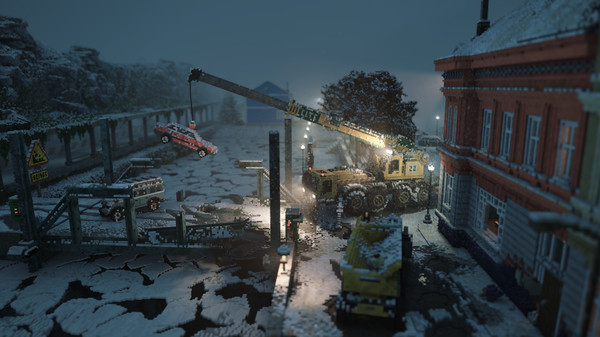
\includegraphics[width=\linewidth]{images/graphics/teardown.jpg}
    \caption{The voxel based sandbox Teardown (2022) by Tuxedo Labs.}
    \label{fig:teardown}
\end{figure}

Tuxedo Labs \emph{Teardown} (figure \ref{fig:teardown}) uses ray traced lighting which is affordable due 
to the voxel scene representation. [@TODO: Check Teardown ray tracing]
Additionally, it makes use of highly dynamic physics operation which are relatively efficient using the voxel 
representation. In their base layout, cubical voxels are \ac{AABB}es which allows for trivial collision tests.
When rotated around any axis, they are still oriented bounding boxes, making collision tests more expensive,
but still rather efficient. These characteristics make voxels excellent candidates for dynamic physics 
calculations. Also, storing voxels in a spatial container helps keep collision checks to a minimum. \\

\noindent
In the next chapter we will focus on the first use case, the Rasterized Voxel Rendering. We belive that this 
technique can benefit the most from advances in rendering technology.
With most of the latest improvements of graphics hard- and software, the capabilities to process mesh data 
and compute a rasterized image got better and better. Even the graphics hardware vendors efforts to enable 
real time ray traced lighting, shadows, reflections and ambient occlusion is applied within the rasterized 
pipeline and therefore relies on improvements to said paipeline over the last years. \\
We will first lay out a technical foundation in chapter \ref{cpt-technical-background} before discussing 
related work on which our approach relies on in chapter \ref{cpt-related-work}.







- Spectrum between CPU computation and GPU computation. 
CPU <-----------> GPU

- Mesh-Shading pipeline as new standard 

- Poses question, can mesh shading further optimize voxel rendering?

- Voxel Rendering

- Better geometry creation (in contrast to Geometry Shader)
- Optimized occlusion culling using per-meshlet OC

    \chapter{Technical Background} \label{cpt-technical-background}


\section{Voxel Rendering} \label{sec-voxel-rendering}


\subsection*{Rasterized Voxel Rendering} \label{subsec-rasterized-voxel-rendering}

The basic approach to rendering voxels is using the traditional rasterized Rendering Pipeline.
One of the most popular games of all time, \emph{Minecraft} (Mojang \cite{Mojang2024}, 2011) uses 
this approach to render thousands of cube shaped voxels on screen. \emph{Minecraft} also makes use 
of various rendering optimizations to improve frame times. This approach is straightforward in 
concept and can be implemented for existing \ac{API}s, making use of hardware acceleration, i.e. 
the \ac{GPU}. The voxel representation allows for easy computations since geometry is laid out 
regularly. Lighting calculations, as well as phyisics operations, can be further optimized to 
be even more efficient. The most significant advantage is the ability to dynamically enable or 
disable voxels within the scene layout. Or, in general, to update voxels and their corresponding 
data efficiently. Also, since voxels are regular shapes, they can be easily created on the \ac{GPU} 
as opposed to being sent over the \ac{PCI Express} port. 


\subsection*{Ray Traced Voxel Rendering} \label{subsec-ray-traced-voxel-rendering}

[@TODO: Add citations for all examples]
A rather common approach to visualization of voxels in 3D space is \emph{ray tracing}. When using 
ray tracing, it is essential to consider different acceleration strategies. The regular and memory 
efficient encoding of voxels allows for fast tracing against the geometry. Another acceleration 
technique is to use \ac{BSP} Trees or similar spatial algorithms which store information about the 
layout of geometry in space. This can help discard parts of a scene which are not of interest for 
the computational process or (e.g. using an \emph{Octree} data structure) store more detailed data in 
one part of a scene, and keep the data resolution low in parts where (almost) no geometry is present. 
Geometry doesn't even have to be present, since voxels can be stored as a bit value, storing either a 
voxel within a given part of the scene (e.g. in a regular grid) (1), or keeping the bit clear (0) if 
no voxel is present at the given location. Ray traced approaches not always make use of the volumetric 
nature of voxel scenes, but often generate voxels only where necessary for faster traversal. A \ac{SVO} 
only stores octree nodes, and therefore voxel data, where there is actually data present, skipping paths 
down the hierarchical structure which are not contributing to the final scene data. Still, ray tracing 
is a very expensive operation, depending on the data that is being computed during each ray sample. 
That means that voxel resolutions have to be adapted according to the use case and hollow models are 
preferrable to restrict the tracing operations to minimum.


\subsection*{Voxel Physics} \label{subsec-voxel-physics}

\begin{figure}[h]
    \centering
    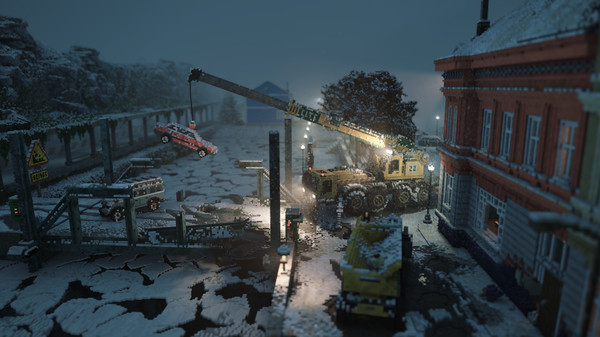
\includegraphics[width=\linewidth]{images/graphics/teardown.jpg}
    \caption{The voxel based sandbox Teardown (2022) by Tuxedo Labs \cite{TuxedoLabs2022}.}
    \label{fig:teardown}
\end{figure}

\noindent
Tuxedo Labs' \emph{Teardown} (figure \ref{fig:teardown}) uses ray traced lighting, which is affordable due 
to the voxel scene representation \cite{TuxedoLabs2022}. Additionally, it makes use of highly dynamic physics 
operations, which are relatively efficient using the voxel representation. In their base layout, cubical 
voxels are \ac{AABB}es which allows for trivial collision tests. When rotated around any axis, a voxel is 
still an \ac{OBB}, making collision tests more expensive, but still rather efficient. These characteristics 
make voxels excellent candidates for dynamic physics calculations. Also, storing voxels in a spatial container 
helps keep collision checks to a minimum.


\section{Voxel Scene Layout} \label{sec-voxel-scene-layout}

The voxel rendering in our evaluation relies on a volumetric representation of the scene.
It is particularly important that the voxel model not only includes the surface but also 
the space within the model. This constraint is often used in interactable use cases, where 
the model is split, cut or manipulated in any given way. \emph{Minecraft} \cite{Mojang2024}
lets the player take full control over the sandbox environment and allows adding or subtracting 
voxels as they wish. Essentially, the voxel data of every possible voxel within the playable 
space needs to be somehow present or encoded in memory, even though just a fraction of the 
voxels are actually drawn to the screen.


\subsection*{Three Dimensional Grid} \label{subsec-three-dimensional-grid}

A basic approach for a scene representation is a three dimensional voxel grid. This 
approach relies on a fixed size grid where each grid cell represents one voxel.
To draw the voxels, a separate buffer can hold additional voxel information, which 
can be accessed by a given grid cell index. The voxel data can store information about 
whether a voxel is present in that particular grid cell or not, which color the voxel 
should have, the normals for lighting calculation and any other data necessary.
This approach is relatively lightweight but inefficent for large grid sizes and low 
grid occupations. All grid cells need to be traversed to draw any given scene which 
might include a lot of empty grid cells. Additionally, storing the voxel data seperately
introduces a pointer indirection on each step of the traversal, potentially leading to more 
cache misses.


\subsection*{Octree Data Structure} \label{subsec-octree-data-structure}

Another approach is to use a spatial container to optimize traversal. The use of an \emph{octree} 
incorporates the relevant scene space and subdivides it into smaller child nodes. When inserting data 
into the octree, the position is evaluated and the data is being stored as a \emph{payload} in 
a node which includes the given position. If a node holds more payload instances than a specified threshold 
allows, it is split into eight child nodes and the payload originally present in the node is 
distributed onto the child nodes. This process is repeated until all data is finally inserted 
into the octree. The resulting octree maintains all the relevant payload data, having a deeper tree 
hierarchy where more data is present and a shallow hierarchy where almost no or no data is present.

\begin{figure}[h]
    \centering
    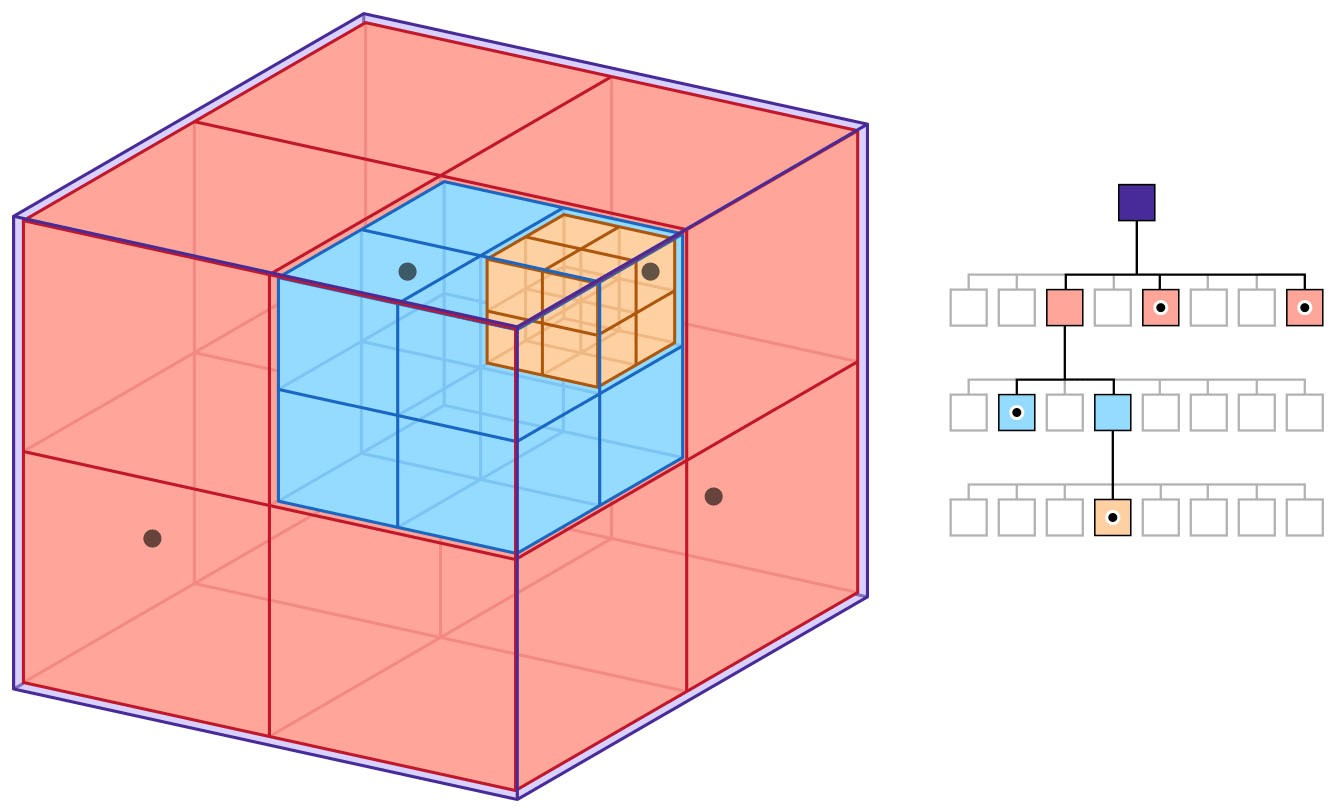
\includegraphics[width=300px]{images/graphics/octree.jpg}
    \caption{An octree data structure. It stores data alongside its spatial characteristics, relative to 
    other data entries \cite{Six2021}.}
    \label{fig:octree}
\end{figure}

\noindent
Octrees like this can vary in their specific implementation, especially in how they maintain the 
payload. Some might store it right next to the octree node description, others might want to separate 
octree and payload data. Octree nodes could also be appended to a dedicated buffer and therefore be stored 
separately from the tree hierarchy description. Such an approach would maintain cache coherency during an 
unordered traversal of all octree nodes. [@TODO: find appropriate sources]\\

\noindent
When using hierarchical data structures, dedicated vertex positions can be omitted and instead 
the voxel position in space can be implicitly calculated from the hierarchy and the root node's bounds. 
This allows for improvement of memory occupation, which is vital for loading and storing high 
resolution voxel scenes. A voxel's state can be encoded into either visible (1) or empty (0).
A bitwise representation of voxels can significantly decrease the memory footprint, that the next 
approach expand on.


\subsection*{High Resolution Sparse Voxel Directed Acyclic Graphs} \label{subsec-highres-svo-dags}

Kampe et al. \cite{Kampe2013} use data redundancy to further generalize and optimize high resolution 
\ac{SVO}s. In their implementation, the octree data structure relies on bitmasks, to encode the existence of child 
nodes. This way, empty nodes are ignored and the information can be easily stored within one byte. This child node 
mask uniquely identifies the layout of the nodes below and can also be used to store the voxel occupation of the 
leaf nodes. Next, they make use of the fact that an octree node's position is uniquely identifed by the path along 
the nodes from root to leaf node. Since voxels can be encoded as either being present or not, and non-present 
voxels can be ignored, the data can be significantly reduced in size. Furthermore, equal child node masks 
can simply be shared between different parent nodes instead of being duplicated. Kampe et al. \cite{Kampe2013} 
suggest a bottom-up approach to remove redundant nodes and replace whole sub-trees of the octree by pointing to one 
instance of the same pattern within the tree, which is shown in figure \ref{fig:sparse-voxel-dag-creation}. 
This optimization can be recursively done to each layer in the tree hierarchy, resulting in an optimized version 
of the data structure. The resulting structure is a more general hierarchical data structure, namely a \ac{DAG}.

\begin{figure}[h]
    \centering
    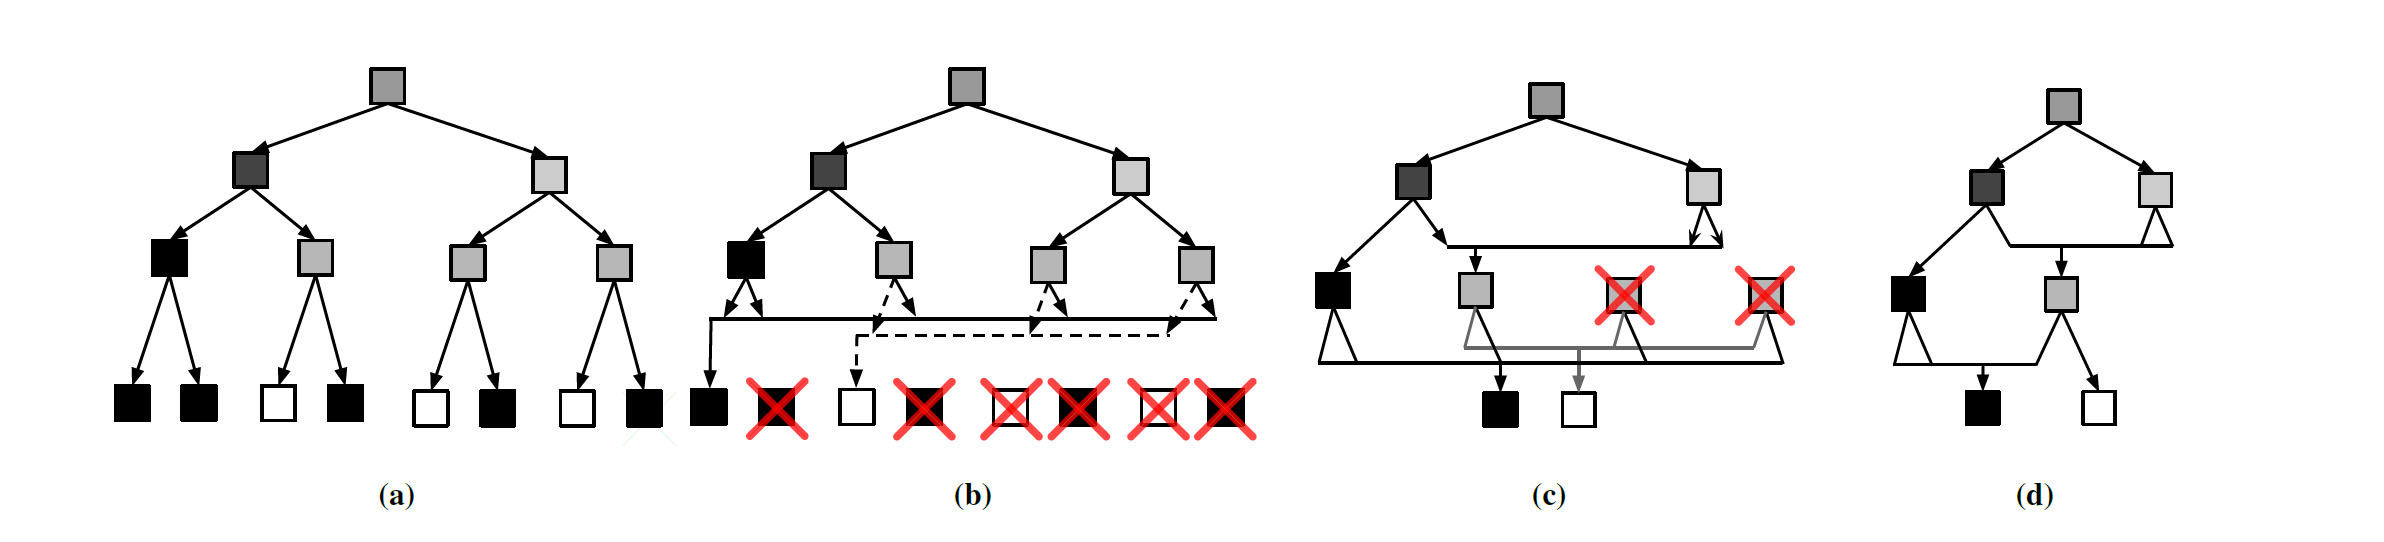
\includegraphics[width=\linewidth]{images/graphics/highres-sv-dag.jpg}
    \caption{Reducing a \ac{SVO} using the approach of Kampe et al. \cite{Kampe2013}.}
    \label{fig:sparse-voxel-dag-creation}
\end{figure}

\noindent
This approach seems to be the best solution for reading, storing and optimizing octree data, although we use 
a more basic approach in our implementation. Nevertheless, this concept of optimizing voxel data is compatible 
with our use case and is highly recommended by us.


\section{Culling Techniques} \label{sec-culling-techniques}

\emph{Culling} refers to the technique to discard parts of a scene "that are not considered to contribute to the final 
image" \cite{AkenineMoeller2018}. This allows for highly populated scenes to be rendered, since most parts of a scene 
will probably not be visible by the camera at the same time. Ignoring culled objects or triangles is therefore a common 
process in real-time rendering. "The fastest triangle to render is the one never sent to the \ac{GPU}" 
\cite{AkenineMoeller2018}. In this section, the most common culling techniques are presented and the ones considered by 
our approach are specifically highlighted and analyzed. 


\subsection*{Backface Culling} \label{subsec-backface-culling}

Backface culling is concerned with discarding triangles that are facing away from the camera. 
These triangles will not be seen by the camera anyway and thus can be safely ignored in the rendering process. 
To compute the facing direction of a triangle, which when normalized is equivalent to the triangle's 
\emph{Surface Normal}, the vertex \emph{winding order} of the given rendering backend is considered.

\begin{figure}[h]
    \centering
    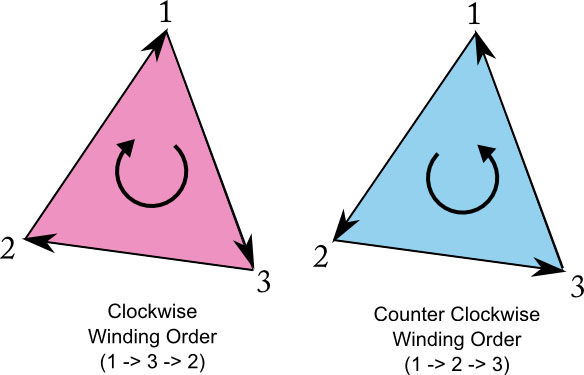
\includegraphics[width=200px]{images/graphics/winding-order-triangle.jpg}
    \caption{Two possible winding orders of triangles \cite{Michel2016}.}
    \label{fig:triangle-winding-order}
\end{figure}

\noindent
When describing a triangle mathematically, the vertex positions are considered, which perfectly define the edges of 
said triangle. The surface can then be interpreted as facing towards the viewer or away from them. 
When trying to compute the triangle, its vertex positions can be recorded in an arbitrary order, but to encode which 
direction the surface is facing, the vertex position order is specified up front. Microsoft's rendering \ac{API}s D3D11 
and D3D12 for example encode a counterclockwise winding order to be interpreted as facing towards the viewer 
\cite{D3DTopology2020}. With this standard in place, all triangles can uniquely define their orientation relative to 
the camera. When enabling backface culling within the rendering backend, triangles which are not facing the camera 
are automatically omitted immediately after screenmapping \cite{AkenineMoeller2018}. Depending on the type of geometry, 
backface culling can remove up to half of the triangles about to be rendered, proving very valuable to highly populated 
scenes and high geometric density.

\begin{figure}[h]
    \centering
    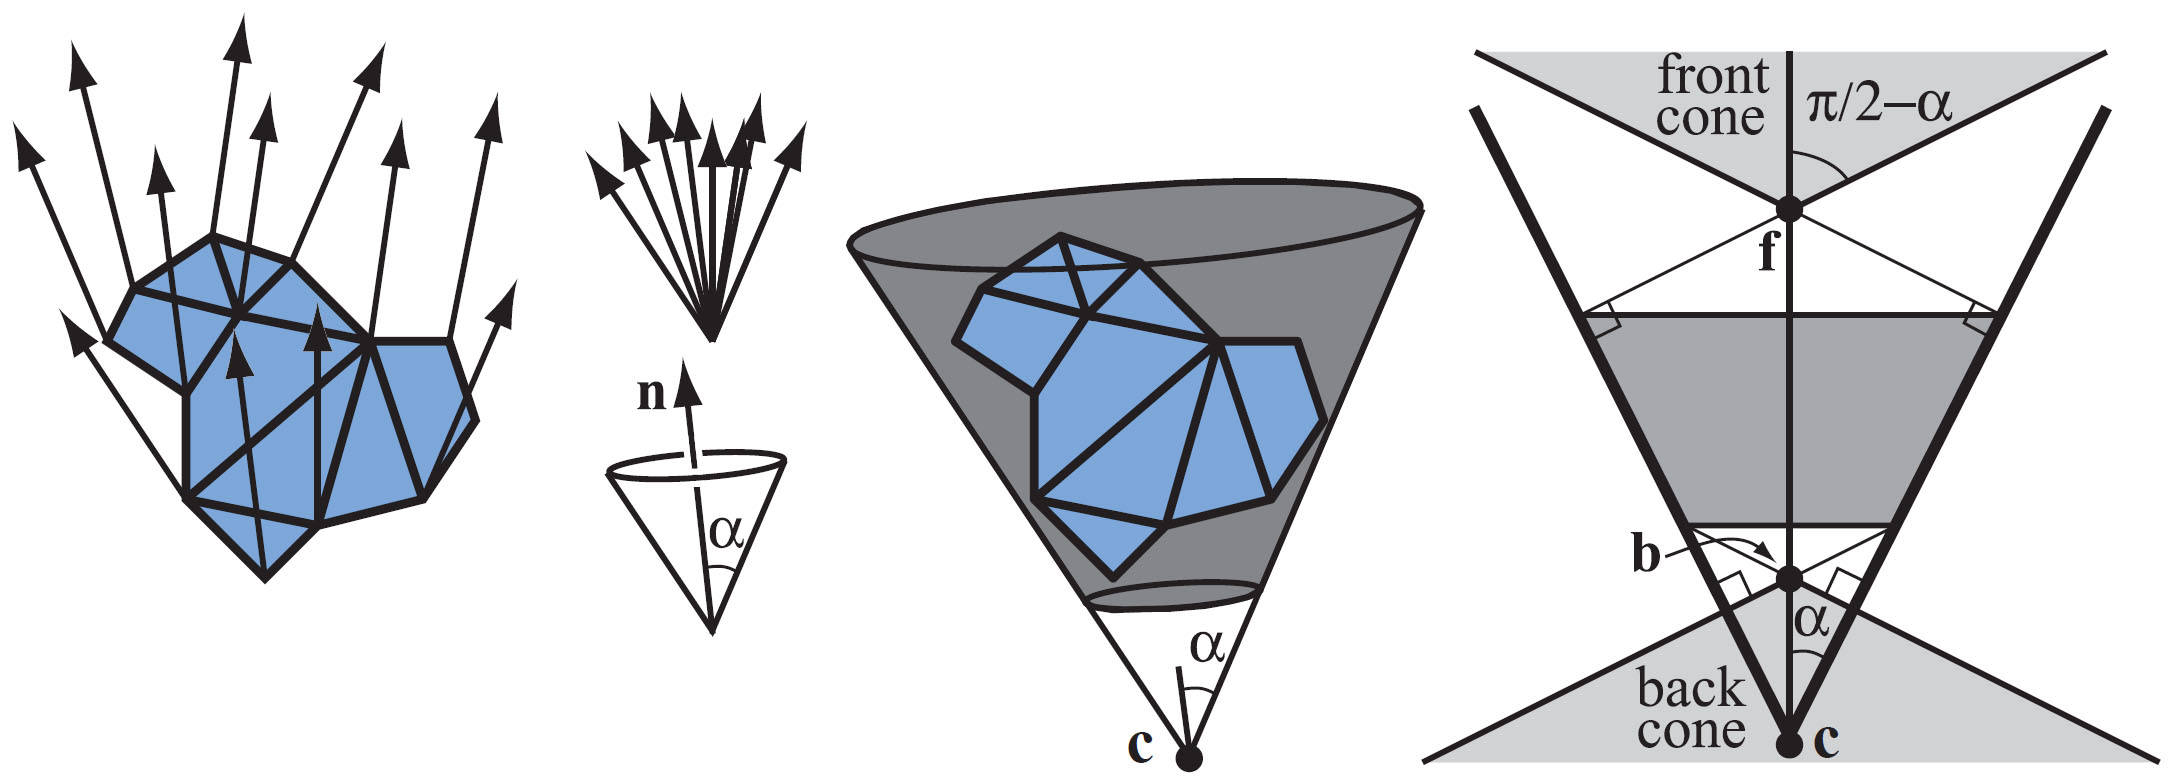
\includegraphics[width=300px]{images/graphics/cluster-backface-culling.jpg}
    \caption{A common normal cone of a triangle cluster. It can be used to calculate a frontfacing
    and a backfacing cone. If the camera is located in either of these cones, all triangles in the 
    cluster are facing toward the camera, or away from it respectively \cite{AkenineMoeller2018}.}
    \label{fig:cluster-backface-culling}
\end{figure}

\noindent 
Backface culling algorithms can also be applied to clusters of triangles. As Shirmun et al. \cite{Shirmun1993} propose, 
multiple triangles can be culled at once considering a common normal cone. "Shirmun and Abi-Ezzi \cite{Shirmun1993} 
prove that if the viewer is located in [a] frontfacing cone [constructed by the normals of all the triangles within the 
cluster], then all faces in the cone are frontfacing, and similarly for the backfacing cone" \cite{AkenineMoeller2018}. 
As will be mentioned in chapter \ref{subsubsec-meshlet-backface-culling}, this approach can be used for more 
parallelized backface culling using an updated rendering pipeline in current graphics \ac{API}s. A visual representation 
is provided in figure \ref{fig:cluster-backface-culling}.


\subsection*{View Frustum Culling} \label{subsec-view-frustum-culling}

\begin{figure}[h]
    \centering
    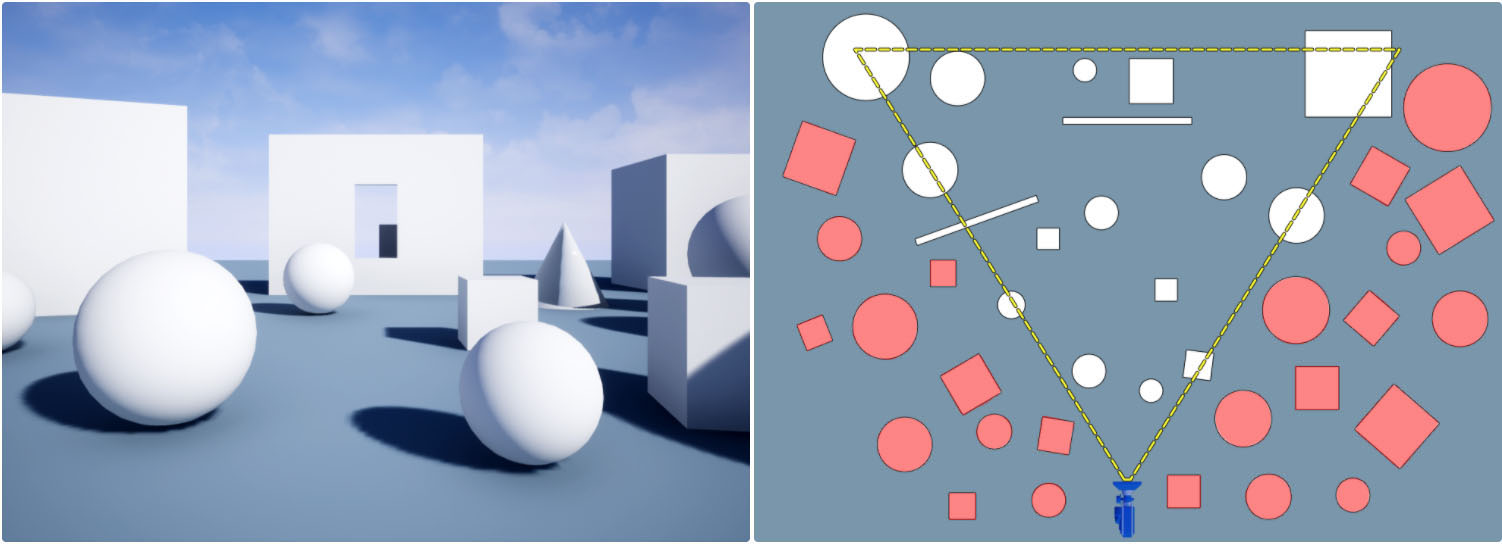
\includegraphics[width=\linewidth]{images/graphics/view-frustum-culling.jpg}
    \caption{The camera's view frustum, relative to the scene. All objects that are completely outside of 
    the view frustum can be ignored by the rendering pipeline, since they do not contribute to the resulting image.
    Image by \cite{Pan2020}.}
    \label{fig:view-frustum-culling}
\end{figure}

\noindent
\emph{View Frustum Culling} is a technique that aims to remove instances, i.e. meshes, which are outside of the camera 
view frustum. This leads to the skipping of all instances that are completely invisible due to their location relative to 
the camera. Said instances can thus be safely ignored and discarded early in order to keep the memory occupation low. 
Figure \ref{fig:view-frustum-culling} shows how the view frustum might look in relation to the scene. 
To cull potantial instances, bounding volumes are calculated and checked against the camera view frustum, which in turn 
is specified by the \emph{near plane} and \emph{far plane}, as well as the \emph{fov}, encoded in a \emph{dot-normal}
representation. For instance, testing if a bounding sphere is partially or completely inside the view frustum can be 
computed with the following algorithm: \\

\fbox{
\begin{minipage}{\linewidth}
\begin{algorithm}[H]
\SetAlgoLined
\KwIn{float4 basePosAndScale}
\KwResult{Boolean indicating whether an object is visible}

\SetKwFunction{FMain}{IsVisible}
\SetKwProg{Fn}{Function}{:}{}
\Fn{\FMain{float4 basePosAndScale}}
{
    float4 center $\gets$ float4(basePosAndScale.xyz, 1.0f)\;
    float radius $\gets$ abs(basePosAndScale.z)\;

    \For{$i \gets 0$ \KwTo $5$}{
        \If{dot(FrustumPlanes[$i$], center) $<$ $-$radius}{
            \Return{false}\;
        }
    }
    \Return{true}\;
}
\caption{Visibility Check Algorithm}
\end{algorithm}
\end{minipage}
}
    
\vspace{0.5cm}
\noindent
In combination with acceleration structures like an octree, view frustum culling can be computed for the bounding 
volumes of the given structure, which can further optimize the culling operations due to spatial grouping of multiple 
instances. This technique is also applied in our approach, using spheres as approximations for the cubical octree 
bounding volumes.


\subsection*{Occlusion Culling} \label{subsec-point-based-occlusion-culling}

When considering highly populated scenes, there might be cases of meshes occluding other meshes. This produces overdraw 
when rasterizing the final projection, which means that multiple color values will be calculated for the same pixel 
before the final color is determined. In general, overdraw should be avoided where possible. Having a lot overdraw 
within the rendering process means that visibility determination of instances is deferred to the last possible point in 
the rendering pipeline. Often, it is better to pre-determine visibility and sample only visible instances. To achieve 
this, algorithms can be used to select and omit occluded instances. \\

\begin{figure}[h]
    \centering
    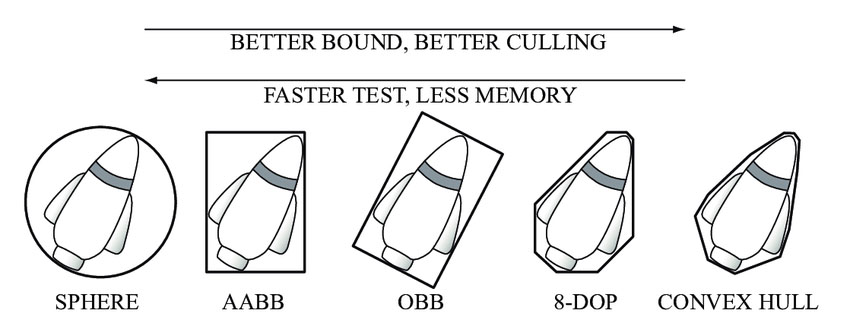
\includegraphics[width=300px]{images/graphics/bounding-volume-quality.jpg}
    \caption{Different bounding volumes provide different advantages and disadvantages \cite{Six2021}.}
    \label{fig:bounding-volumes}
\end{figure}

\noindent
Different occlusion culling algorithms can be applied depending on scene layout, object characteristics and other factors.
As it is the case with culling algorithms in general, occlusion culling algorithms usually rely on bounding volumes to 
approximate object positions and scale in space. Figure \ref{fig:bounding-volumes} shows how different bounding volumes 
can be used to support faster computation or more accurate volume approximation. Algorithms have been proposed which 
operate in \emph{image space}, \emph{object space} or \emph{ray space}, with image space occlusion culling being most 
widely adopted in real-time rendering \cite{AkenineMoeller2018}. These algorithms operate on a projected 2D image to 
consider visibility of different instances.  


\subsubsection*{Hierarchical Z-Buffering} \label{subsubsec-hierarchical-z-buffering}

\emph{\ac{HiZ} Buffering} is a technique first introduced for \ac{CPU} computation by Ned Greene et al. 
\cite{Greene93,Greene95}. Since then, it "has had significant influence on occlusion culling research" 
\cite{AkenineMoeller2018}. It is a fundamental basis on which our approach relies on, which will be discussed 
in more detail.\\


[@TODO: explain texel (?), mip levels]
\begin{figure}[h]
    \centering
    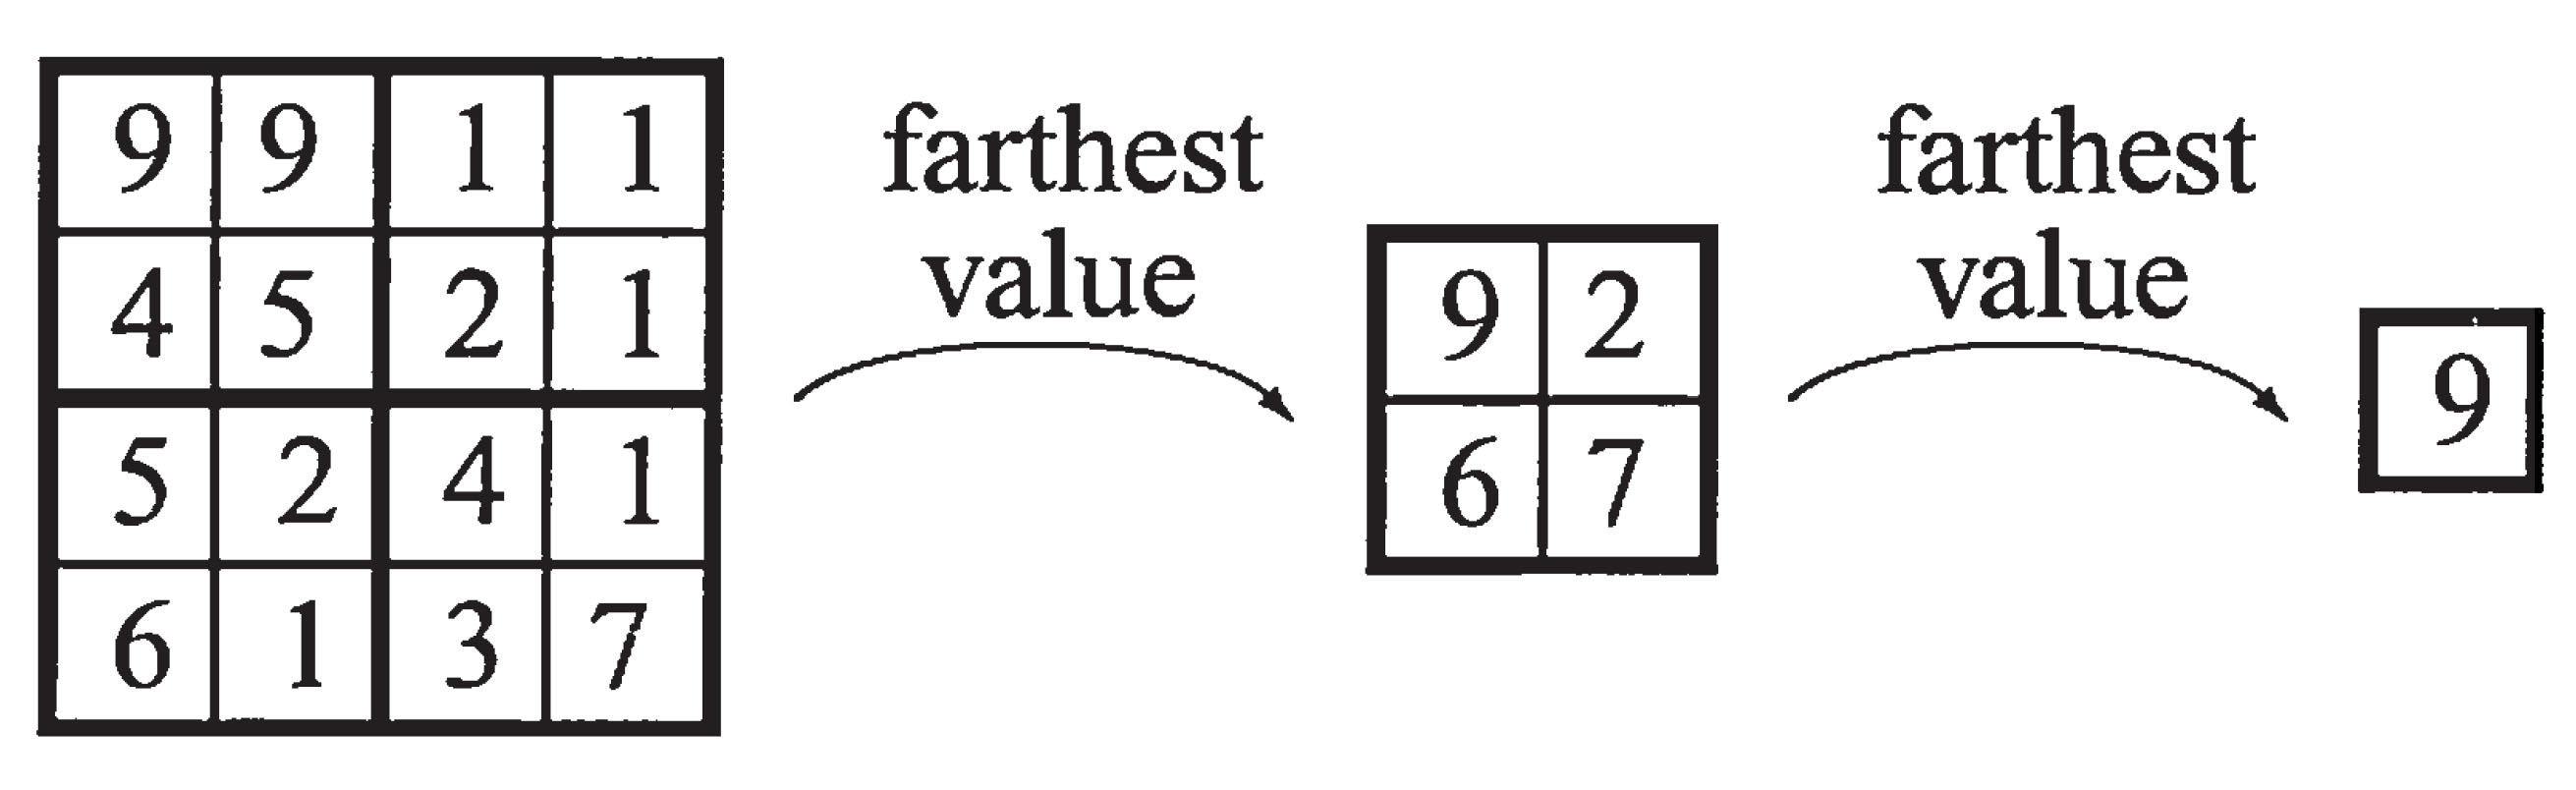
\includegraphics[width=200px]{images/graphics/hiz-buf-values.jpg}
    \caption{The calculation of a \ac{HiZ} buffer computes the farthest value of each texel window, 
    resulting in a new texel value for adjacent mip levels \cite{AkenineMoeller2018}.}
    \label{fig:hiz-value-computation}
\end{figure}

\noindent
\ac{HZB} is computed in image space and relies on two main components. An octree scene representation and a 
\emph{z-buffer} pyramid. [@TODO: Check if z-buffer or mip-map needs to explained] 
The octree contains all instances present in the scene. The \emph{z-pyramid} is a set of z-buffer mip-maps, with every 
map reducing in size relative to the previous mip-map. The reduction is computed by aggregating values from 4 texels 
within the previous mip-map and writing the output value into one texel of the new mip-map level. This way, both axes 
(u and v) are scaled to be half the length of the previous level. The resulting z-pyramid then has the full resolution 
z-buffer as the finest granularity in the z-pyramid and a very low resolution and small texture on the other end. 
An exemplary z-pyramid is shown in figure \ref{fig:hiz-mip-chain}.\\

\noindent
The computation of new values is another crucial step. "[...] [E]ach z-value is the farthest z in the corresponding 
2 \begin{math}\times\end{math} 2 window of the adjacent finer level" \cite{AkenineMoeller2018}. This process is shown 
in figure \ref{fig:hiz-value-computation}, showing how the farthest value of each texel window is inserted into adjacent 
levels.\\

\begin{figure}[h]
    \centering
    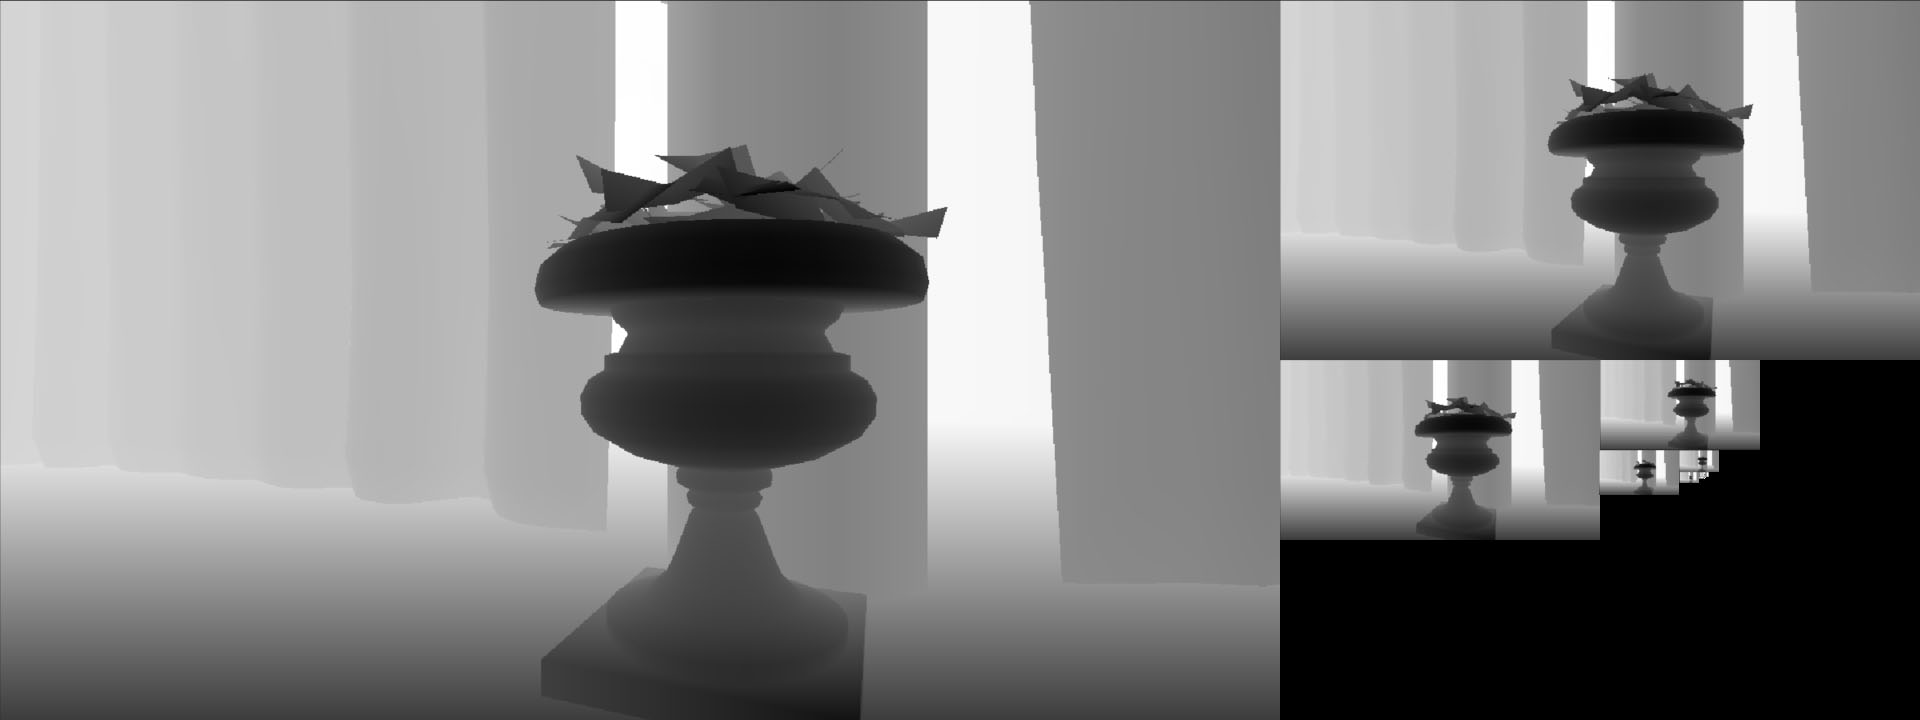
\includegraphics[width=\linewidth]{images/graphics/hiz-mip-chain.jpg}
    \caption{A mip chain of a scene's z-buffer. Every buffer in this chain is a quarter of the resolution of its 
    predecessor buffer \cite{Schachtschabel2017}.}
    \label{fig:hiz-mip-chain}
\end{figure}

\noindent
A visibility test against this z-pyramid is computed as follows: The octree is traversed in a front to back order 
and each octree node is transformed into image-space, essentially projecting the bounding volume of the node onto 
the view plane. Now, the projected bounding volume overlaps a specific region of the view plane, which is then 
tested against the coarsted z-pyramid cell, containing this volume projection. The nearest z value of the bounding 
volume is compared to the z-pyramid's farthest value entries. If the bounding volume's z happens to be farther than the 
\ac{HiZ} value, it is consequently occluded. If the comparison yields the opposite result, the test "is continued 
recursively down the z-pyramid until the [bounding volume] is found to be occluded, or until the bottom level of the 
z-pyramid is reached, at which point the box is known to be visible" \cite{AkenineMoeller2018}. Visibile octree nodes 
are then drawn to the depth buffer, meaning all the geometry contained within the node is drawn to the depth buffer 
for being tested against during the computation of the following octree nodes. As Akenine-Möller et al. 
\cite{AkenineMoeller2018} point out, this algorithm is not used in its original form. Modern variations of this 
algorithm evolved from the work of Greene et al. \cite{Greene93} and are widely adopted in modern real-time computer 
graphics. As will be shown in chapter \ref{subsubsec-two-pass-occlusion-culling}, the concept of an octree representation 
used for hierarchical culling and a z-pyramid used as an occlusion representation (\cite{AkenineMoeller2018}) can be 
elegantly leveraged on the \ac{GPU} side for efficient occlusion culling.


\subsubsection*{Two-Pass Occlusion Culling} \label{subsubsec-two-pass-occlusion-culling}

\begin{figure}[h]
    \centering
    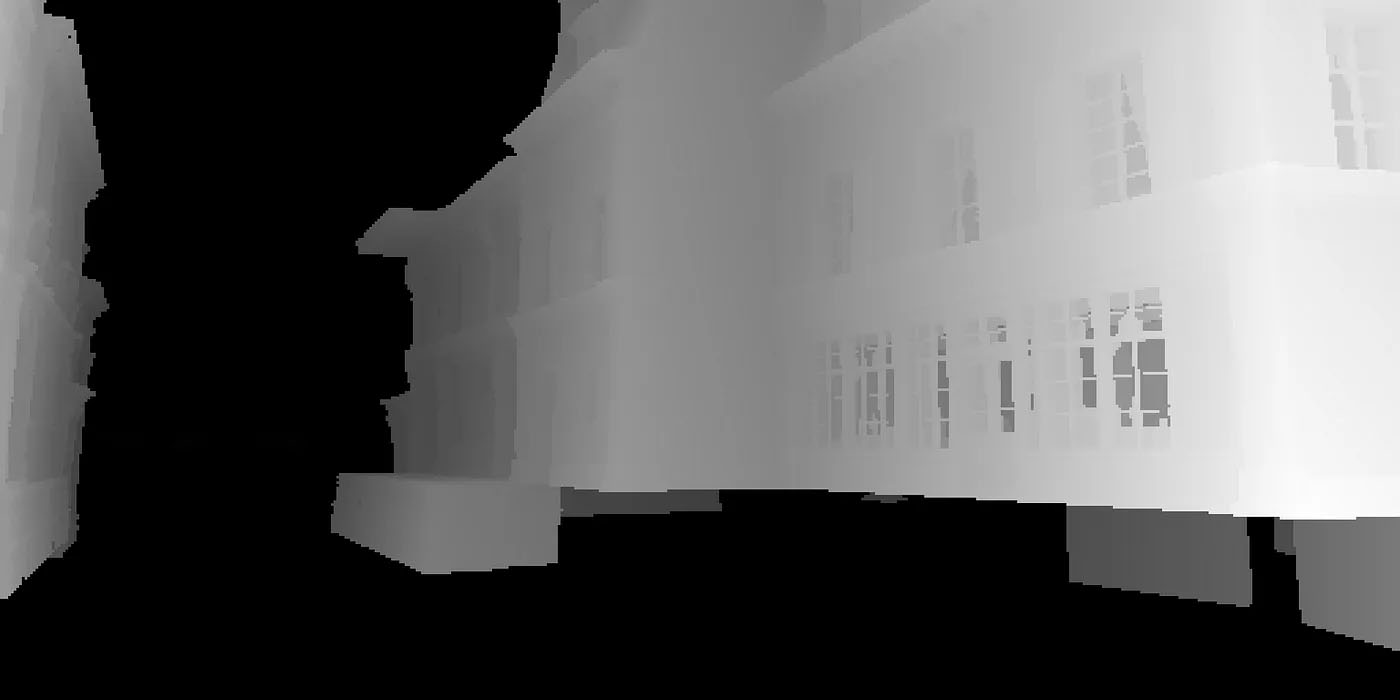
\includegraphics[width=200px]{images/graphics/depth-buffer-ac-unity.jpg}
    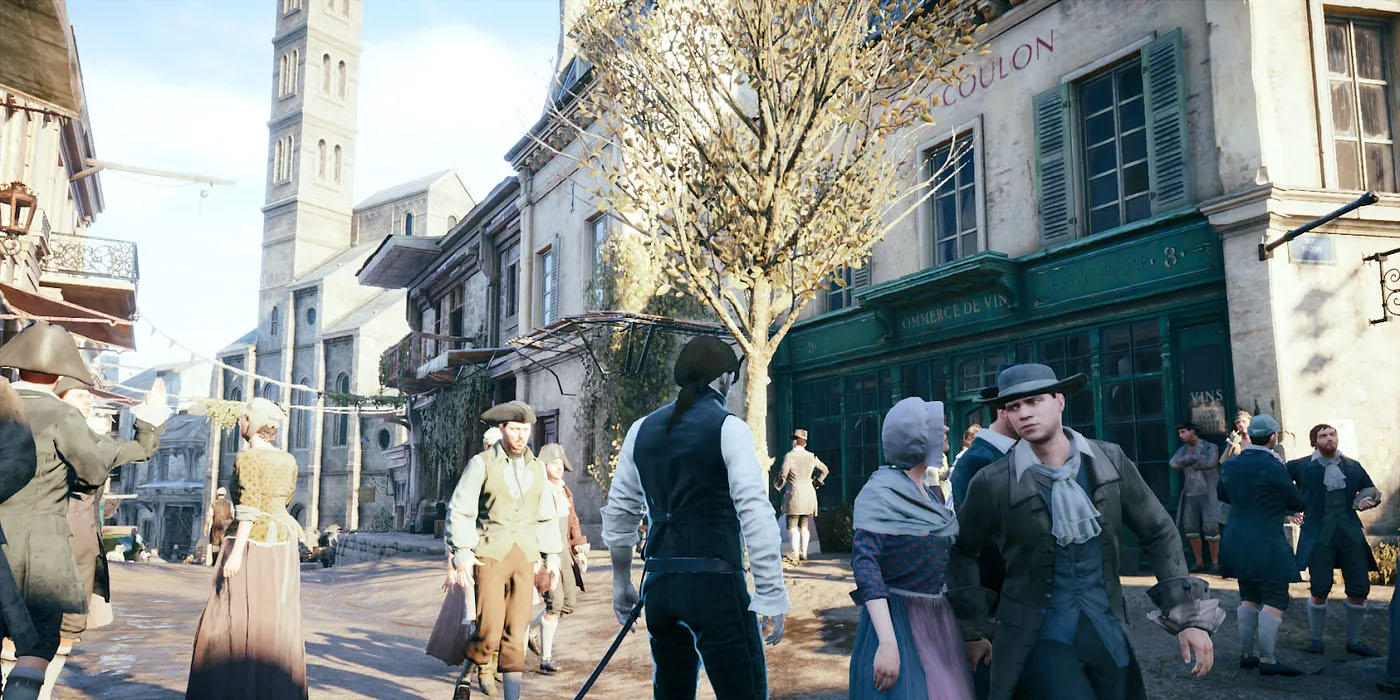
\includegraphics[width=200px]{images/graphics/final-frame-ac-unity.jpg}
    \caption{The depth buffer (left) and the final back buffer (right) of \emph{Assassin's Creed Unity} (\emph{Ubisoft}, 2014 \cite{Ubisoft2014}). 
    The hand-picked \emph{best occluders} were already drawn to the depth buffer in a depth pre-pass.
    While rendering all the geometry to the back buffer, each instance can be checked against the z-pyramid \cite{Kruskonja2022}.}
    \label{fig:depth-buffer-ac-unity}
\end{figure}

\noindent
\emph{\ac{TPOC}} is an adaptation of the \ac{HZB} algorithm, introduced in chapter \ref{subsubsec-hierarchical-z-buffering}. 
One of the most renowned examples of this algorithm is present in the 2014 title \emph{Assassin's Creed Unity} by \emph{Ubisoft} 
\cite{Ubisoft2014}. One year later, Ulrich Haar and Sebastian Aaltonen presented their approach on SIGGRAPH 2015 
\cite{Aaltonen2015}. Their implementation inspired other developers like \emph{Epic Games} for \emph{Unreal Engine 5} 
to adopt similar techniques \cite{Karis2021}. This is the algorithm we use in our implementation. It shares its basic 
principle with \ac{HZB} but focuses on a more \ac{GPU}-driven configuration and using a given set of best occluders to 
cull instances effectively. \\

\noindent
Some use cases are especially well suited for \ac{TPOC}, \emph{Assassin's Creed Unity} for example has a large open 
world in a city with many large buildings. A rather large amount of instances can therefore be expected to be occluded 
by some of the buildings at any given moment. \ac{TPOC} thus uses artist-picked \emph{best occluders} for \ac{HZB} 
computation. The best occluders are identified during runtime, drawn to depth buffer during a depth pre-pass, and 
then used as described in chapter \ref{subsubsec-hierarchical-z-buffering}. The output of the depth buffer pre-pass is 
shown in figure \ref{fig:depth-buffer-ac-unity}. Depth passes can be done quite efficiently, especially if they 
only contain a handful of instances to draw. Additionally, because of the advances in \ac{GPU}-driven Rendering, the 
\ac{HiZ} pyramid can be computed by a \emph{compute shader}, which leverages the highly parallel computation 
capabilities of the \ac{GPU}. \\

\noindent
In contrast to the basic \ac{HZB}, this approach relies on the heavy use of \ac{GPU} computation and the pre-
determination of best occluders. This way, the scene doesn't have to be reversed in a front to back order and 
not necessarily needs to incorporate an octree, as long as object bounds can be computed efficiently enough.
In SIGGRAPH 2015 presentation, Aaltonen et al. \cite{Aaltonen2015} mention the addition of another acceleration 
technique, which is compatible with \ac{TPOC}, \emph{Depth Reprojection}.


\subsubsection*{Depth Reprojection} \label{subsubsec-depth-reprojection}

\emph{Depth Reprojection} makes use of the temporal coherence of the z-buffer. The assumption is made that 
between two consecutive frames most of the visible content remains the same. It is obvious that this will 
hold true for the most part when the camera's rotation and position isn't changed inbetween frames. In this case, 
the last frames depth, color and visibilty information would remain nearly identical. The only differences would 
be introduced by animation or physics simulation, which could move instances independently from the camera movement.
But even with the camera moving over frames, a large part of the scene - static parts like buildings or terrain in 
particular - would retain a lot of its information. This means that there will be a significant coherence in 
visibility between frames, which Depth Reprojection makes use of.\\

\noindent
The algorithm stores the last frame's depth information and "reprojects" it onto the new frame. In the best case, 
most instances, which were previously visible remain visible in this new frame, and instances, which were invisible 
in the previous frame remain invisible in the new frame as well. The new camera transformations and a 
\emph{Velocity Vector Buffer} are used to calculate the delta relative to the previous frame and create an 
approximation of the new depth buffer. Because the reprojected depth buffer is only an approximation, visibility 
and depth calculations can be inprecise, because the result is non-conservative. This means that the reprojection 
process sometimes fails to compute the correct depth values for objects, especially if they move relative to the 
camera. Another problem occurs in use cases, where the camera moves very fast relative to the environment. In such 
a case, the camera might cover a too large distance, so that none of the visible instances in a given frame were 
visible during the previous frame. \cite{Kruskonja2022} \\

\noindent
The \ac{TPOC} algorithm is used in our approach, with minimal changes to the selection of best occluders.
Depth Reprojection could in general be used as well, but is not within the scope of our implementation.


\section{Mesh Shading}  \label{sec-mesh-shading}

Mesh Shaders were first introduced to NVIDIA Turing \ac{GPU}s in 2018 as a part of "a new programmable 
geometric shading pipeline" and built upon the compute programming pipeline \cite{Kubisch2018}. 
Therefore, they aim to optimize work by using the available hardware more efficiently. Compared to the 
traditional vertex shading pipeline, mesh shading introduces a more holistic and parallel processing of 
geometry data. It is incorporated into the rasterized rendering pipeline and has since been used in modern 
gaming. It gained a lot of attention when it was used as the foundation of Epic Games' \emph{Unreal Engine 5} 
feature \emph{Nanite} \cite{Karis2021}.\\


\subsection*{Mesh Shading Pipeline} \label{subsec-the-mesh-shading-pipeline}

In contrast to the \emph{Mesh Shading Rendering Pipeline}, the "traditional" \emph{Vertex Shading Pipeline} 
has more specialized stages, which are listed in figure \ref{fig:traditional-rendering-pipeline}. This pipeline 
is composed of fixed, programmable and optional stages, where each stage operates on some input data and in 
some cases produces output data for the next stage to consume.\\

\begin{figure}[h]
    \centering
    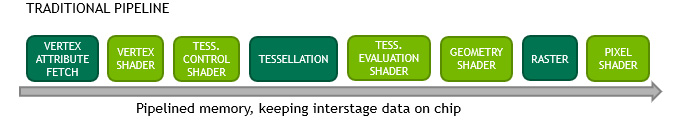
\includegraphics[width=\linewidth]{images/graphics/traditional-rendering-pipeline.jpg}
    \caption{The traditional rendering pipeline as presented by NVIDIA in \cite{Kubisch2018}.}
    \label{fig:traditional-rendering-pipeline}
\end{figure}

\noindent
The \emph{Vertex Attribute Fetch} stage (also called \emph{Input Assembler} stage) collects the geometric 
input and creates primitives out of it, reading all necessary data associated with the primitive data. 
These primitives are usually triangles but this can vary slightly from use case to use case, depending
on the prior configuration of the stage. After the Input Assembler, the data is sent to the \emph{Vertex Shader}.
This stage is responsible for operating on single vertices, transforming vertices according to the given 
transformation matrices. After that, the \emph{Tesselation Control Shader} can optionally increase geometric 
resolution or triangulate polygonal geometry by applying tesselation functions. The next stage is the optional 
\emph{Geometry Shader}, which is capable of generating additional primitives on the \ac{GPU}. However, it is 
commonly said to be not very efficient and is treated as deprecated since the introduction of the more general 
purpose and faster \emph{Compute Shaders} [@TODO: source]. The three-dimensional scene is then projected onto the 
view plane and is subsequently processed by the \emph{Rasterizer} which samples the continuous lines and faces to 
find the appropriate pixels covered by the geometry. Finally, the final frame buffer is colored correctly by the 
\emph{Pixel Shader}. This stage takes all given parameters like light position, light color, light intensity, camera 
position, vertex colors, textures and many more into account and creates a final, colored image. The pixel shader can 
implement different functions (\ac{BRDF}) for calculation of the final pixel color and is called once per pixel. 
This means, that the computational cost increases with the amount of pixels, i.e. the frame buffer's resolution. 

\begin{figure}[h]
    \centering
    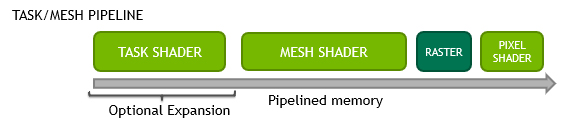
\includegraphics[width=\linewidth]{images/graphics/mesh-rendering-pipeline.jpg}
    \caption{The mesh shading pipeline as presented by NVIDIA in \cite{Kubisch2018}.}
    \label{fig:mesh-rendering-pipeline}
\end{figure}

\noindent
The \emph{Mesh Shading Rendering Pipeline} is a rendering pipeline, optimized for high geometrical 
density. It shares the Rasterizer and the Pixel Shader stages with the Vertex Shading Pipeline but 
introduces two new stages which aim to replace the Vertex Shader, Geometry Shader and Tesselation stage.
The new stages are called \emph{Task Shader} (or \emph{Amplification Shader}) and \emph{Mesh Shader}. Both 
are fully programmable and are based on the compute shader architecture. Therefore, they are inherently different 
from the traditional Vertex Shader stage, even though they both can be used for vertex transformations.
Figure \ref{fig:mesh-rendering-pipeline} shows the pipeline stages and the order they are executed in. \\

\noindent
The Task Shader serves as a precomputational stage which is optional and invokes the Mesh Shader.
It can take any arbitrary data as input and operates on the provided data to produce output data, which is then 
scheduled for further computation. Since both shaders are based on compute shaders, a threadgroup size can be 
specified  and groupshared memory can be allocated. This allows for highly parallelized execution and optimized 
memory usage. A key difference to the traditional pipeline is that the Amplification Shader can invoke other 
compute shaders, create new tasks and dispatch none, one, or multiple mesh shader invocations. This makes the 
shader extremely flexible and capable of providing the same results as the Geometry Shader does, but faster and 
more scalable. It is often used for early culling, for efficient tesselation or \ac{LOD} decisions \cite{Kubisch2018}. \\

\begin{figure}[h]
    \centering
    
\includegraphics[width=300px]{images/graphics/bunny-meshlet.jpg}
    \caption{The \emph{Stanford Bunny} mesh geometry split into meshlets. Each meshlet is represented by a single color, 
    and consists of multiple triangles \cite{Oberberger2024}.}
    \label{fig:bunny-meshlet}
\end{figure}

\noindent
The Mesh Shader output can be defined individually but usually it creates a small patch consisting of a small 
number of triangles, called \emph{Meshlet}, which are shown in figure \ref{fig:bunny-meshlet}. This new approach 
to operate on vertices allows for a new interpretation of mesh data. The primitive topology is not anymore constrained 
to triangles, triangle fans and triangle strips, but can be individually specified by the developers.
Meshlets are computed by threadgroups which usually fetch the mesh data from the given vertex and index buffers and 
apply transformations and arbitrary operations. This new way of processing geometry is not only more efficient in many 
cases and reduces the memory bandwidth, but also allows for per-meshlet operations \cite{Kubisch2020}. This is a key 
advantage, since per-instance geometry can now be processed in parallel and still be individually discarded or post-processed. 
There are several other advantages over the traditional Vertex Shaded Pipeline, which we will not list to the full 
degree. More details are provided in the blog post by NVIDIA \cite{Kubisch2020}.\\


\subsection*{Meshlet Culling} \label{subsec-meshlet-culling}

One major innovation that is enabled by the use of Mesh Shading is to cull on a per-primitive (per-meshlet) basis. 
This allows for more granular culling of high density geometry even within instances. Prior to the implementation 
of meshlets, culling usually was done on a per-instance basis (or for backface culling on a per-triangle basis), 
omitting whole instances depending on their position in space or their visibility from the point of view of the camera.\\

\noindent
But although the Mesh Shading Pipeline was first introduced in 2018, the idea of triangle clusters goes back even further.
One example of this \ac{GPU}-driven rendering technique is the 2014 title \emph{Assassin's Creed Unity} \cite{Ubisoft2014}.
Aaltonen et al. \cite{Aaltonen2015} provide an overview over multiple cluster related optimization techniques, implementing 
a highly parallelized rendering pipeline before Mesh Shading became part of the official Rendering \ac{API}s.
For their \ac{GPU} culling algorithms they refer to the prior work of Hill \cite{Hill11} and Greene \cite{Greene93}, which 
provides the basis for some of the implementation in our case study. Most of the culling algorithms discussed in chapter 
\ref{sec-culling-techniques} can be adopted to use meshlet culling. The algorithms can usually be applied to triangle clusters 
without the need of changing a lot of the algorithm. Bounding volumes can be calculated for meshlets, too, and meshlets do also 
consist of triangles themselves. In this chapter we briefly revisit the basic culling algorithms and show, how they can be 
adapted for the Mesh Shading pipeline.


\subsubsection*{Meshlet Backface Culling} \label{subsubsec-meshlet-backface-culling}

As shown in chapter \ref{subsec-backface-culling}, there are backface culling algorithms which can be applied to 
triangle clusters as well. For instance, the normal cone approach by Shirmun et al \cite{Shirmun1993} can be used 
in the Mesh Shading pipeline as well. In fact, having a hardware and software support for the computation of triangle 
clusters makes this approach even more efficient. Clusters are evaluated in parallel, making a normal cone backface 
culling algorithm very fast. \\

\noindent
Another algorithm compatible with triangle clusters is the one propsed by Aaltonen et al. \cite{Aaltonen2015}, again 
in the context of the SIGGRAPH 2015 presentation, showing their work for \emph{Assassins Creed Unity}. They introduce 
a small bounding cube around \emph{n} triangles, which could correspond to a meshlet in the Mesh Shading pipeline. 
"Each cube face is split into \emph{r} \begin{math}\times\end{math} \emph{r} 'pixels', each encoding an \emph{n}-
bit mask that indicates whether the corresponding triangle is visible over that 'pixel'" \cite{AkenineMoeller2018}.
As long as the camera is outside of the cube, the center of the cube creates a frustum with any of the "pixels" on 
the cube's surface, as shown in figure \ref{fig:backface-culling-ac-unity}. The frustum in which the camera is 
located can be found and the bitmask can be accessed. This way, the backfacing triangles can be identified and 
culled. \cite{Aaltonen2015}, \cite{AkenineMoeller2018}

\begin{figure}[h]
    \centering
    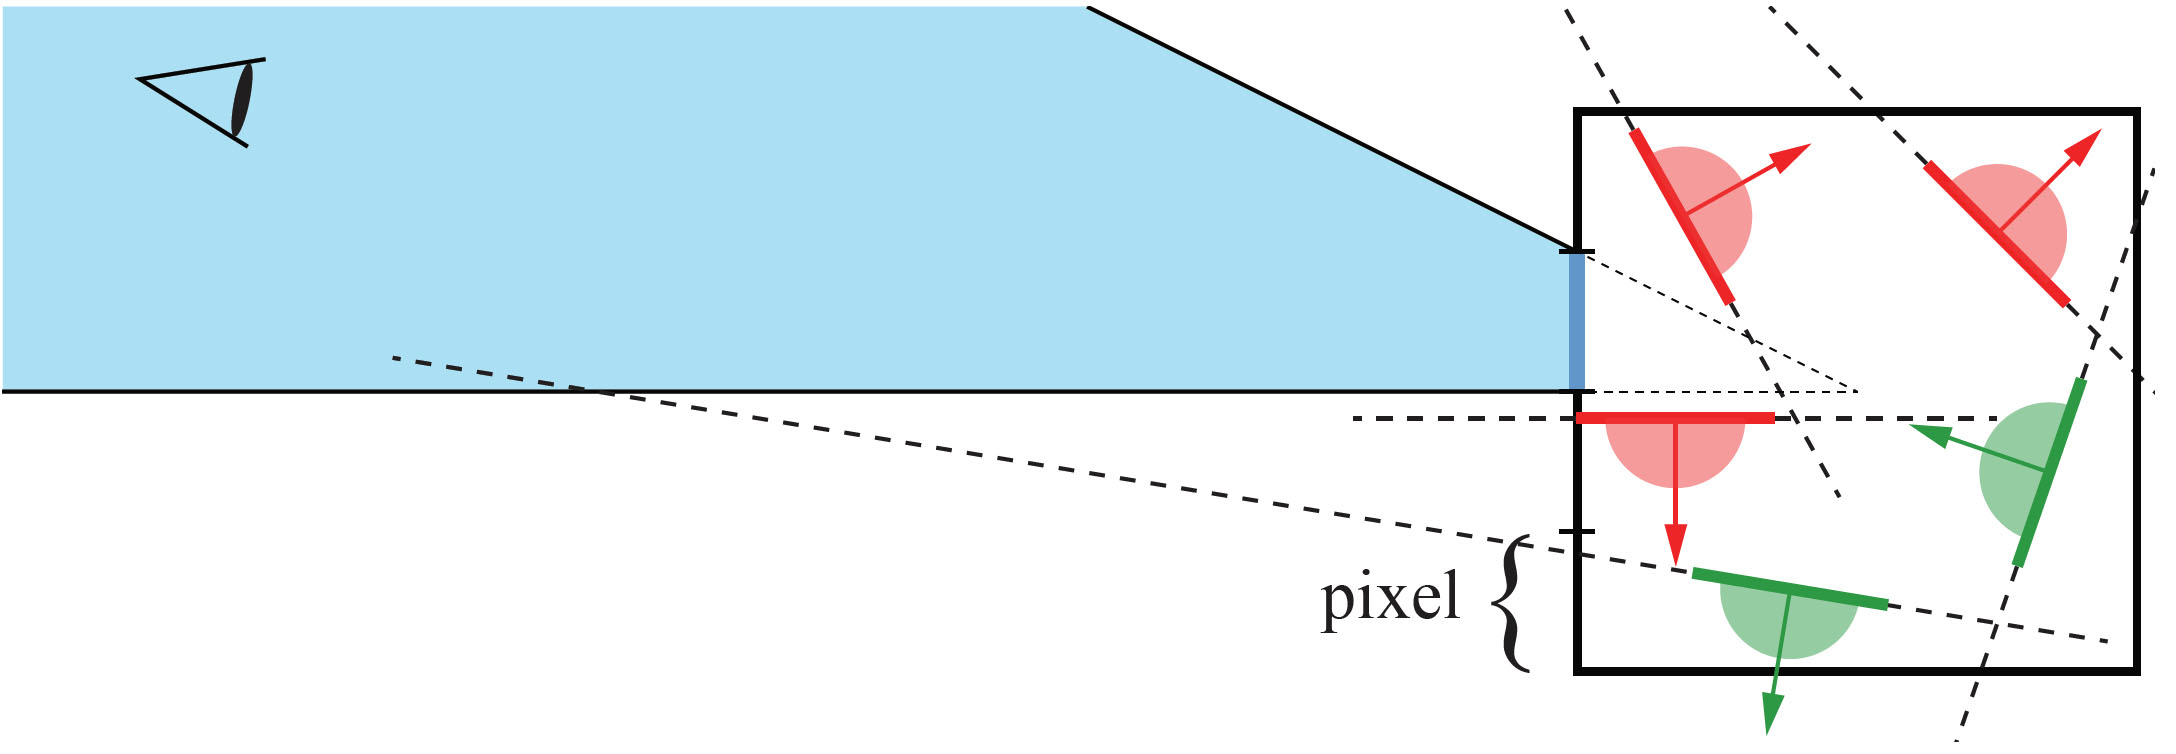
\includegraphics[width=\linewidth]{images/graphics/backface-culling-ac-unity.jpg}
    \caption{Backface culling thechnique using a bounding box around a set of \emph{n} triangles, 
    as proposed by Aaltonen et al. \cite{Aaltonen2015}. Image by Akenine-Möller et al. \cite{AkenineMoeller2018}.}
    \label{fig:backface-culling-ac-unity}
\end{figure}


\subsubsection*{Meshlet View Frustum Culling} \label{subsubsec-meshlet-view-frustum-culling}

[@TODO: Check if pre-calculated meshlets have been introduced; find sources]
Frustum culling can be adapted to work on meshlets as well. Similar to backface culling, the basic technique remains 
the same, but is applied to triangle clusters (meshlets) rather than instances (meshes). To implement this, meshlet 
bounding volumes need to be computed. The same principles apply to meshlet bounding volumes as to instance bounding 
volumes, so spherical volumes are usually fast and cheap to calculate. If the meshlets are pre-calculated, the 
bounding volumes can be precalculated as well, since they will not change over time. Then, frustum culling is as simple 
as using any existing frustum culling algorithm (see \ref{subsec-view-frustum-culling}) and applying it to the meshlets.
Since this can be done in the Task Shader, the culling can be computed in parallel and culled meshlets can be discarded 
early. This includes parts of single instances, which allows for even better optimization. In the traditional Vertex 
Shading pipeline, instances had to be completely outside of the view frustum in order to be culled. If an instance is 
partially visible in the Mesh Shading pipeline, the meshlets inside the frustum can be drawn and the meshlets outside 
of the frustum can be discarded. \\

\noindent
We use view frustum culling of individual meshlets in our approach to further optimize performance. A simple 
implementation was already included in the framework we used for our case study.


\subsubsection*{Meshlet Occlusion Culling} \label{subsubsec-meshlet-occlusion-culling}

Meshlet occlusion culling refers to the process of culling meshlets which are occluded by any other meshlet, by a 
group of meshlets or another instance. This culling technique is rather new due to the relative novelty of the 
Mesh Shading pipeline itself. Still, Aaltonen et al. \cite{Aaltonen2015} used what they call \emph{Cluster Culling} in 
\emph{Assassin's Creed Unity} (\emph{Ubisoft} \cite{Ubisoft2014}, 2014). Meshlet occlusion culling can be implemented in 
a bunch of different ways, exactly as traditional occlusion culling algorithms. Often, this implies the use of a 
\ac{BVH} like an octree to make visibilty checks easier. \ac{HZB} can also be applied to the new pipeline, and meshlets 
can be checked for occlusion, using the highly parallel Mesh Shading pipeline. Consequently, \ac{TPOC} is also applied 
to individual meshlets, as seen in Alan Wake 2 (Remedy Entertainment \cite{Remedy2023}, 2023) or Epic Games' 
\emph{Unreal Engine 5} and \emph{Nanite} \cite{Karis2021}.\\

\noindent
We believe that this new way of culling single meshes can generate new innovation in the field of computer graphics.
This is why we decided to implement our approach in a Mesh Shading pipeline, which, when used carefully, is more 
efficient than comparable methods like the use of Geometry Shaders or Instancing.
    \chapter{Related Work} \label{cpt-related-work}

\section{Octree Occlusion Culling}



\section{Alan Wake / Northlight}

- What is it?
- What is interesting about it?
- How does it relate to our work?
- How does it differ from our work?

    \chapter{Evaluation} \label{cpt-evaluation}


    \chapter{Case Study}

% @TODO: Meshlet Creation -> Voxel

- Meshlet creation for voxel meshes is trivial since meshlets don't have to be per-computed
- Meshlezt culling is also straight forward since Voxels are inherently AABBs
- 
    \chapter{Results} \label{cpt-results}

- Results of the case study
    \chapter{Discussion} \label{cpt-discussion}


- Pro: 
    - No meshlet precomputation, since meshlets are created on the GPU
    - Meshlet voxels are inherently AABBs which is quite helpful for intense intersection computations % @TODO: Check if there are even any intersection comps to be done

- Con:
    - Depending on the voxel size, there might be a need for chunking the data effectively % @TODO: Check if this is still necessary with Meshlet Occlusion Culling enabled
    - Voxels as meshlets -> non-similar normals can be inefficient.. 
    - 


Discussion points:

- When already drawing aggregated bounding boxes, isn't this just HiZ Buffering? And is it then better to draw everything
 to test for visibility instead of only best occluders? 
    \chapter{Prospect} \label{cpt-prospect}



\section{Future work}

- Use every thread in threadgroup and do not leave threadgroups idle when rejecting nodes (View Frustum Culling or frustum culling)
- Use Sparse Voxel DAGs and better data compression
- Use meshlet backface culling technique
- The construction of the \ac{HiZ}-pyramid can possibly be further optimized by computing values for all mip levels 
  in parallel, instead of sequentially writing and reading the values to or from a given mip level. 
- Test runtime performance when updating the best occluders dynamically. E.g. apply physics operations to voxels models.
- Use raster occlusion approach \cite{NVIDIAGLOC2016} instead of \ac{HiZ}.
    
    \chapter{Conclusions}

    % ********************************************************************
    % End of contents
    % ********************************************************************
    
    \cleardoublepage
    \printbibliography
    \cleardoublepage
    \addchap{List of Acronyms} % Abkürzungsverzeichnis


\begin{acronym}[SPS] % longest acronym in [...] for spacing
    % \acro{short}{long}
    % \acroextra{...} wird nur im Abkürzungsverzeichnis ausgegeben.
    \acro{ISW}{Institut für Steuerungstechnik der Werkzeugmaschinen und Fertigungseinrichtungen \acroextra{der Universität Stuttgart}}
    \acro{SPS}{Speicherprogrammierbare Steuerung}
    % acrodefplural, wenn eine Pluralform benötigt wird (Standard: angehängtes "s" aus dem Englischen)
    % \acrodefplural{acroKey}[plural short]{plural long}
    \acrodefplural{SPS}[SPS]{Speicherprogrammierbare Steuerungen}
    \acro{NDA}{Non-Disclosure Agreement}

\end{acronym}
    
    \cleardoublepage
    \listoffigures
    
    \cleardoublepage
    \listoftables
    
    \cleardoublepage
\addchap{List of Symbols}

This section is optional. 
Ask your supervisor whether it is required for your thesis. 
If you have more than 10 formulas involved it probably is.

There are two ways to build a list of symbols:

\begin{itemize}
    \item If you just want to get it done, then use a \texttt{longtable} and fill your symbols in, see table below.
    \item If you want it fancy, then package \texttt{glossaries} (maybe \texttt{glossaries-extra}) may be your way to go. 
    Be warned that although it automates symbol handling (e.g. sorting and referencing of symbols), it comes with some administrative overhead. 
    You can find a discussion on different ways to achieve this \href{https://tex.stackexchange.com/a/366282}{on https://tex.stackexchange.com/a/366282}.
\end{itemize}

\begin{center}
\begin{longtable}{@{}c l p{10cm}@{}}
\toprule
Symbol & Unit & Description \\
\midrule
\endfirsthead
\multicolumn{3}{c}{\textit{List of Symbols -- continued}}\\
\toprule
Symbol & Unit & Description \\
\midrule
\endhead
\bottomrule \multicolumn{3}{r}{\textit{Continued on next page}} \\
\endfoot
\bottomrule
\endlastfoot

% start here with your symbols:
\(\psi\) & rad & Heading angle of hamster \\
\(\dot x\) & m/s & Linear velocity of hamster \\
\(\ddot x_0\) & m/s$^2$ & Initial acceleration of hamster \\
\end{longtable}
\end{center}
    
    % Appendix, if needed:
    \appendix
    \chapter{Appendix (e.g. source code)}


\end{document}